\documentclass[14pt]{extarticle}
\usepackage[english,ukrainian]{babel}
\usepackage[utf8]{inputenc}
\usepackage{amsmath,amssymb}
\usepackage{parskip}
\usepackage{graphicx}
\usepackage{xcolor}
\usepackage{tcolorbox}
\tcbuselibrary{skins}
\usepackage[framemethod=tikz]{mdframed}
\usepackage{chngcntr}
\usepackage{enumitem}
\usepackage{hyperref}
\usepackage{float}
\usepackage{subfig}
\usepackage{chngcntr}
\usepackage{esint}
\usepackage{subfig}
\usepackage[top=2.5cm, left=3cm, right=3cm, bottom=4.0cm]{geometry}
\usepackage[table]{xcolor}
\usepackage{algorithm}
\usepackage{algpseudocode}
\usepackage{listings}
\tcbuselibrary{theorems}

\newtcbtheorem[number within=section]{def}{Визначення}%
{colback=blue!5,colframe=blue!35!black,fonttitle=\bfseries}{th}

\title{Додаткове завдання}
\author{Студента 3 курсу групи МП-31 Захарова Дмитра}
\date{\today}

\begin{document}

\maketitle

Намалювати траєкторії цієї системи
\[
xy^2 + \frac{x^3}{3}-x = C
\]

Траєкторії зображені на рисунку \ref{fig:1} (див. наступну сторінку). 
\begin{figure}[H]
    \centering
    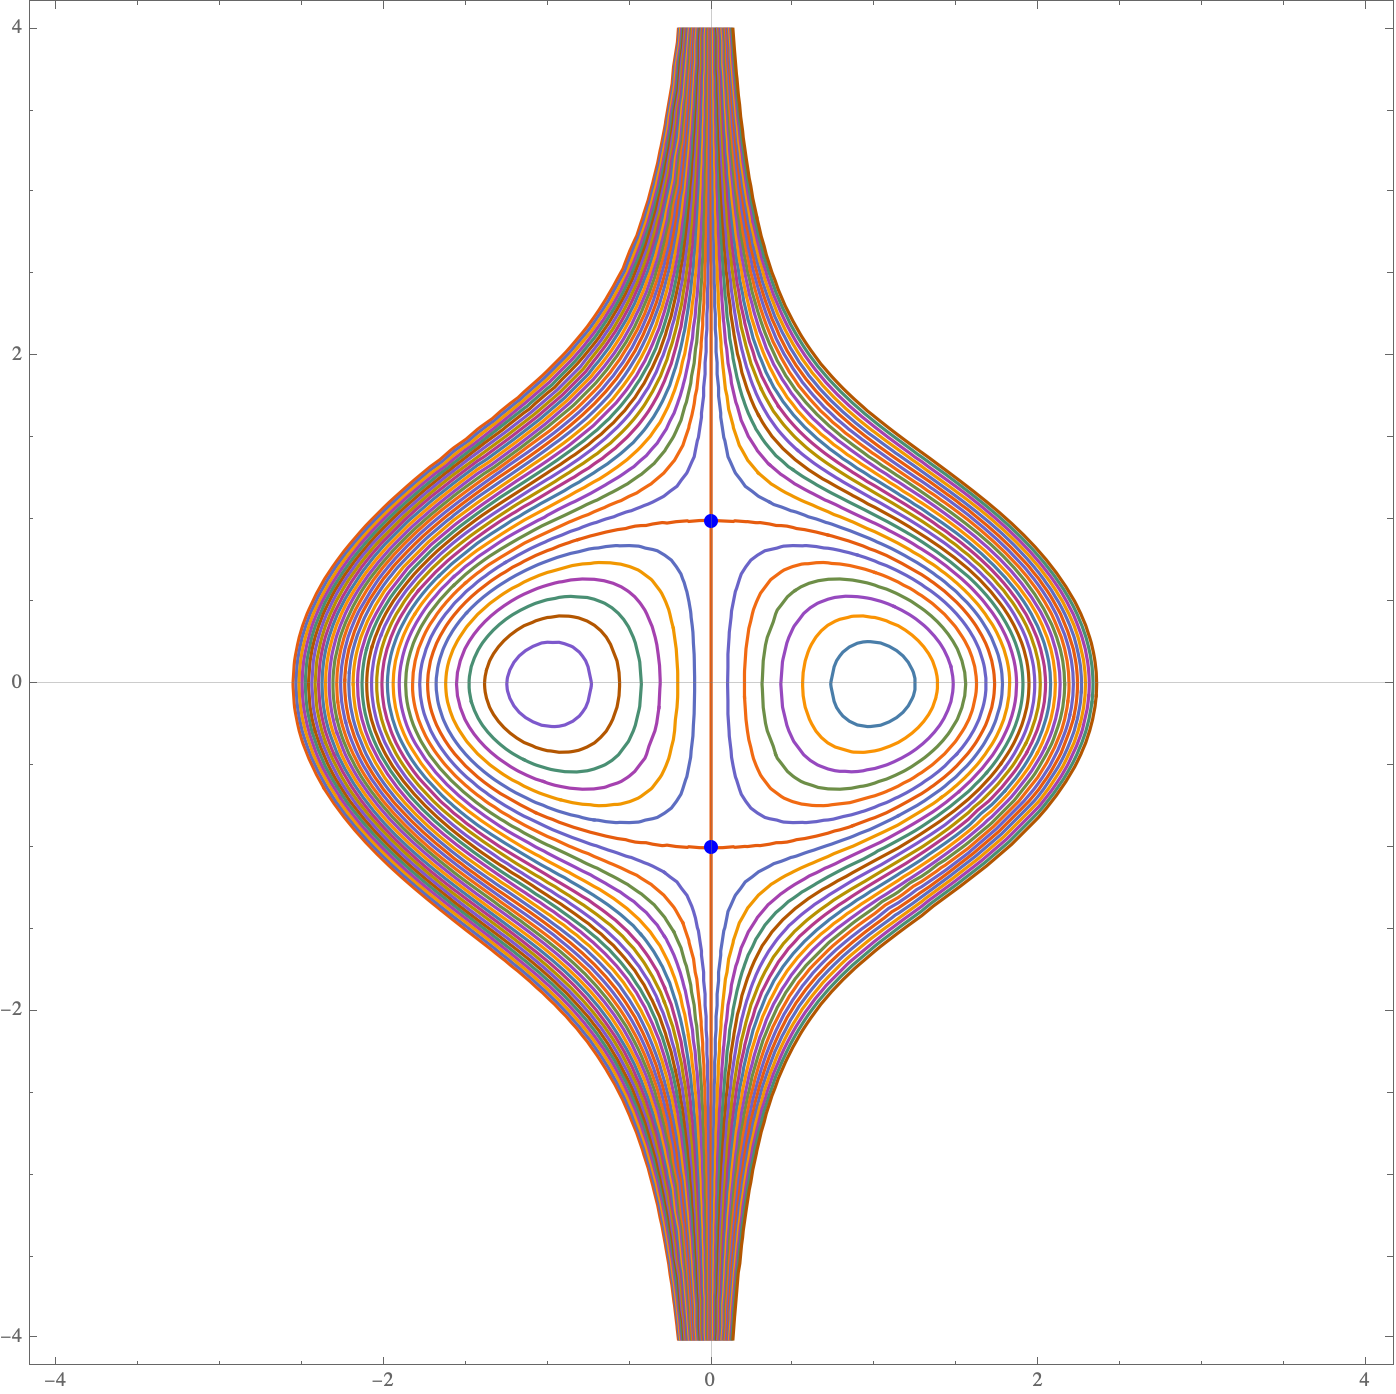
\includegraphics[width=\textwidth]{images/addition/additional_diff_eq.png}
    \caption{Сімейство кривих $xy^2 + \frac{x^3}{3}-x = C$ для $C\in [-3,2]$}
    \label{fig:1}
\end{figure}

\end{document}

